% Copyright 2026 Sreeram Anil
% SPDX-License-Identifier: CC-BY-4.0
% =============================================================================
%  Reduced-order EKF (3-state ECM) — robust_kalman family
% =============================================================================
\providecommand{\vf}{\bm{f}} \providecommand{\vh}{\bm{h}}
\providecommand{\vd}{\bm{d}} \providecommand{\mM}{\bm{M}}
\providecommand{\va}{\bm{a}} \providecommand{\vb}{\bm{b}}

\chapter{Reduced-order EKF (ReducedOrder-EKF)}
\label{ch:reducedorderekf}

\section*{At a glance}
\begin{tabular}{@{}l>{\raggedright\arraybackslash}p{0.76\textwidth}@{}}
Family & Robust / embedded Kalman \\
Header & \texttt{include/estkit/battery/ecm\_model\_reduced.hpp}
         (+ \texttt{filters/ekf.hpp}) \\
Registered name & \texttt{ReducedOrder-EKF} \\
State dimension & $n_x = 3$: $[\soc, v_1, h]$; the slow RC branch is quasi-static \\
Cost per step & $\mathcal{O}(n_x^3)$; 331\,ns/step, 4272\,B, no heap \\
Primary references & \cite{simon2006,plett2016bms2,plett2004ekf2,chen2020parameterization} \\
\end{tabular}

\section{Motivation and aerospace/BMS relevance}
A BMS runs its cell estimator once per cell per sample.  A 100-cell aircraft pack at 10\,Hz is
1000 filter updates per second on a microcontroller that is also doing contactor logic, CAN
traffic, thermal management and isolation monitoring; and because the covariance recursion is
$\mathcal{O}(n_x^3)$, every state removed from the model is worth roughly
$1-(1-1/n_x)^3\approx 3/n_x$ of the estimator's whole budget.  Reducing the model order is
therefore the highest-leverage optimisation available, far more effective than micro-optimising the
linear algebra.

The question is which state to remove.  The 2-RC equivalent-circuit model
\cite{plett2004ekf2,plett2016bms2} carries a fast branch ($\tau_1\approx5$\,s) and a slow branch
($\tau_2\approx120$\,s).  The fast branch must stay: its time constant is comparable with the
mission's power transients, and its voltage is what separates an ohmic drop from an SOC change on
the time scale at which the measurement is informative.  The slow branch is different.  Over
$\tau_2=120$\,s the OCV itself moves by several percent of SOC on this mission, so the terminal
voltage cannot separate $v_2$ from $\ocv(\soc)$: $v_2$ is, for practical purposes, unobservable.
A filter that carries it as a state spends $n_x^3$ arithmetic on a quantity it is not actually
estimating --- it is propagating it open loop and adding noise to it.

Simon's Chapter~10 \cite[Ch.~10]{simon2006} formalises this as \emph{reduced-order Kalman
filtering}: remove the weakly observable states from the estimator, reconstruct them
deterministically, and account for the reconstruction error by an additional noise term.  Plett
\cite[\S3]{plett2016bms2} arrives at the same place from the battery side when discussing how many
RC pairs an ESC model needs.  This chapter implements the reduction as a \emph{model}, not as a
filter, so that the generic \code{Ekf<Model>} of the classical Kalman family is reused unchanged.

\section{Problem statement and assumptions}
The full estimator model of Chapter~\ref{ch:ecm} is
\begin{align}
\soc_{k+1}&=\soc_k+g(i_k)\,i_k, & g(i)&=-\eta(i)\dt/(3600\,Q), \label{eq:ro-z}\\
v_{1,k+1}&=a_1 v_{1,k}+R_1(T)(1-a_1)i_k, & a_1&=e^{-\dt/\tau_1(T)}, \label{eq:ro-v1}\\
v_{2,k+1}&=a_2 v_{2,k}+R_2(T)(1-a_2)i_k, & a_2&=e^{-\dt/\tau_2(T)}, \label{eq:ro-v2}\\
h_{k+1}&=a_h h_k+(a_h-1)\sgn i_k, & a_h&=e^{-|\eta i\gamma\dt/(3600 Q)|}, \label{eq:ro-h}\\
y_k&=\ocv(\soc_k,T_k)+M h_k-v_{1,k}-v_{2,k}-R_0(T_k)i_k. & & \label{eq:ro-y}
\end{align}
The reduced model keeps $\vx=[\soc,v_1,h]^\T$ ($n_x=3$) and removes $v_2$ from the state, replacing
it by the deterministic, input-driven signal
\begin{equation}
\boxed{\;v^{\mathrm{qs}}_{2,k+1}=a_2\,v^{\mathrm{qs}}_{2,k}+R_2(T_k)(1-a_2)\,i_k,
\qquad v^{\mathrm{qs}}_{2,0}=0.\;}
\label{eq:ro-qs}
\end{equation}
\eqref{eq:ro-qs} is \emph{exactly} \eqref{eq:ro-v2} with the feedback path from the measurement
removed: it is a first-order low pass of $R_2(T)\,i$ with the branch's own time constant --- the
quasi-static reconstruction of the slow polarisation.

\begin{assumption}[What the reduction costs]\label{as:ro-cost}
Let $e_{2,k}=v_{2,k}-v^{\mathrm{qs}}_{2,k}$ be the reconstruction error.  It is zero when (i) the
initial condition is known ($v_{2,0}=0$ after a rest, which the benchmark guarantees) and (ii) the
parameters $R_2,\tau_2$ are exact.  It is non-zero and coloured when the parameters are wrong, and
it appears additively in the output equation \eqref{eq:ro-y}.  Following
\cite[Ch.~10]{simon2006} it is modelled as an extra white measurement noise of variance
$\sigma_{v2}^2$,
\begin{equation}
\mR = \sigma_v^2 + \big(R_0(T)\sigma_i\big)^2 + \sigma_{v2}^2 .
\label{eq:ro-R}
\end{equation}
\end{assumption}

\begin{remark}[Why this is not just ``drop a state'']\label{rem:ro-notdrop}
Simply deleting $v_2$ from \eqref{eq:ro-y} would introduce a systematic voltage bias of up to
$R_2 i=180$\,mV at the hover current, which the filter would convert into an SOC error of
$0.25$.  The quasi-static reconstruction \eqref{eq:ro-qs} removes that bias entirely; what remains
is only the \emph{estimation} error of the slow branch, which was small anyway because $v_2$ was
never really estimated.
\end{remark}

\section{Derivation}

\subsection{Observability argument}
Write the measurement sensitivity of the full model,
$\mH=[\partial\ocv/\partial\soc,\,-1,\,-1,\,M]$.  The columns for $v_1$ and $v_2$ are identical,
so a single voltage sample cannot separate them at all; they are separated only by their different
dynamics, i.e.\ by the difference in how $a_1$ and $a_2$ propagate the same input.  Over a window
of $N$ samples the observability of the pair is governed by
\begin{equation}
\mathcal{O}_N=\sum_{k=0}^{N-1}\begin{bmatrix}a_1^k\\a_2^k\end{bmatrix}
                              \begin{bmatrix}a_1^k&a_2^k\end{bmatrix},
\qquad
\operatorname{cond}(\mathcal{O}_N)\ \text{large when}\ a_1^N\ \text{and}\ a_2^N\ \text{are both}\approx1 .
\label{eq:ro-obs}
\end{equation}
With $\dt=0.1$\,s, $a_1=0.9802$ and $a_2=0.99917$: after $N=100$ samples (10\,s, the correlation
time of the mission's gust process) $a_1^N=0.135$ but $a_2^N=0.920$.  The slow branch is still
essentially constant over the window in which the measurement is informative, so it is
indistinguishable from a slowly drifting OCV, i.e.\ from $\soc$ itself.  Estimating it therefore
buys nothing and risks the estimator trading SOC error against $v_2$ error.

\subsection{Reduced Jacobians}
With $\vx=[\soc,v_1,h]^\T$,
\begin{equation}
\mF=\begin{bmatrix}1&0&0\\0&a_1&0\\0&0&a_h\end{bmatrix},
\qquad
\mH=\Big[\tfrac{\partial\ocv}{\partial\soc}(\soc,T)\;\;-1\;\;M\Big],
\qquad
\mB_{:,i}=\begin{bmatrix}g(i)\\R_1(T)(1-a_1)\\ \tfrac{\partial a_h}{\partial i}(h+\sgn i)\end{bmatrix},
\label{eq:ro-jac}
\end{equation}
and the process noise, as in the full model, is the current-sensor noise mapped through $\mB$ plus
a diagonal floor,
\begin{equation}
\mQ=\mB_{:,i}\mB_{:,i}^\T\sigma_i^2+\diag(q_{\mathrm{floor}}^2).
\label{eq:ro-Q}
\end{equation}
Both Jacobians are analytic, which matters: \eqref{eq:ro-qs} is advanced inside $\vf$, so the model
must never be differentiated numerically (that would call $\vf$ many times per step and corrupt
$v^{\mathrm{qs}}_2$).  This restriction is stated in the header and is the reason the reduced model
is registered with \code{Ekf} and not with a sigma-point filter.

\subsection{Flop and memory accounting}
Let $c_3$ be the dominant cubic cost of one EKF cycle.  With $n_y=1$ the EKF spends, per step,
$\mF\mP\mF^\T$ ($2n_x^3$), the Joseph form ($3n_x^3$ including $\mI-\mK\mH$), and
$\mathcal{O}(n_x^2)$ for the gain and the state update.  Reducing $n_x$ from 4 to 3 therefore scales
the dominant terms by $(3/4)^3=0.42$.  The RAM that depends on $n_x$ is
\begin{equation}
n_x(\text{state})+n_x^2(\mP)+n_x n_y(\mK)+n_y(\veps)+n_y^2(\mS)
=\begin{cases}26\ \text{Reals}=208\,\text{B}, & n_x=4,\\
              17\ \text{Reals}=136\,\text{B}, & n_x=3,\end{cases}
\label{eq:ro-mem}
\end{equation}
a $35\,\%$ reduction.  The \emph{total} object is dominated by the OCV lookup table
($2\times241$ \code{Real}s $=3856$\,B), which on a real MCU lives in flash and is shared by all
cells; the measured \code{sizeof} figures (4336\,B versus 4272\,B) therefore understate the saving
by a large factor.  The honest statement is: \emph{per-cell RAM} falls from 208\,B to 136\,B and
per-cell CPU time falls by $31\,\%$ (measured 478\,ns $\to$ 331\,ns).

\section{Algorithm}
The algorithm is the standard EKF; only the model changes.  The one
non-obvious element is the internal quasi-static state:

\begin{algorithm}[H]
\caption{ReducedOrder-EKF --- one sampling period}
\begin{algorithmic}[1]
\Require $\xplus_{k-1}\in\real^3,\Pplus_{k-1},v^{\mathrm{qs}}_{2,k-1},\vu_{k-1},\vy_k,\vu_k$
\State \textbf{Time update:} $\mF\gets$ \eqref{eq:ro-jac} at $\vu_{k-1}$
\State $\soc\gets\soc+g(i_{k-1})i_{k-1}$;\;
       $v_1\gets a_1v_1+R_1(1-a_1)i_{k-1}$;\;
       $h\gets a_hh+(a_h-1)\sgn i_{k-1}$
\State $v^{\mathrm{qs}}_{2,k}\gets a_2 v^{\mathrm{qs}}_{2,k-1}+R_2(T_{k-1})(1-a_2)i_{k-1}$
       \Comment{Eq.~\eqref{eq:ro-qs}, \emph{once} per step}
\State $\Pminus_k\gets\mF\Pplus_{k-1}\mF^\T+\mQ_k$; symmetrise
\State \textbf{Measurement update:}
  $\hat{y}\gets\ocv(\soc,T_k)+Mh-v_1-v^{\mathrm{qs}}_{2,k}-R_0(T_k)i_k$
\State $\mR\gets\sigma_v^2+(R_0\sigma_i)^2+\sigma_{v2}^2$ \Comment{Eq.~\eqref{eq:ro-R}}
\State $\mS\gets\mH\Pminus_k\mH^\T+\mR$;\;
  $\mK\gets\Pminus_k\mH^\T\mS^{-1}$;\;
  $\xplus_k\gets\xminus_k+\mK(\vy_k-\hat{y})$
\State $\Pplus_k\gets(\mI-\mK\mH)\Pminus_k(\mI-\mK\mH)^\T+\mK\mR\mK^\T$; symmetrise; \code{constrain}
\Ensure $\xplus_k,\Pplus_k,v^{\mathrm{qs}}_{2,k}$
\end{algorithmic}
\end{algorithm}

\section{Application to the battery model}
The reduced model exposes the same interface as \code{EcmModel}: $n_x=3$, $n_u=2$, $n_y=1$, index
constants \code{IZ}$=0$, \code{IV1}$=1$, \code{IH}$=2$, \code{u\_of}, \code{x0}, \code{P0},
\code{constrain}, and the optional \code{params()}/\code{set\_params()} for
$\vtheta=[Q,R_0]$, so it can be dropped into any filter in the library that does not evaluate
$\vf$ more than once per step.  $\mP_0=\diag(\sigma_{z0}^2,(2\,\text{mV})^2,0.5^2)$, i.e.\ the full
model's $\mP_0$ with the $v_2$ row and column deleted.

The one new tuning parameter is $\sigma_{v2}$ of \eqref{eq:ro-R}.  Its registered value, 2\,mV,
is the same order as the voltage-sensor noise, and is justified as follows: with exact parameters
the reconstruction error is identically zero, and the dominant contributor is the $\tau_2$
mismatch.  On \texttt{param\_mismatch} ($\tau_2$ scaled by $1.5$) the slow branch reaches
$R_2 i(1-e^{-75/120})=84$\,mV at the end of the take-off hover in the true cell and
$R_2 i(1-e^{-75/180})=61$\,mV in the estimator: a 23\,mV discrepancy at the worst moment of
the mission, decaying to a few millivolts in cruise.  A 2\,mV allowance therefore covers ordinary
operation without making the filter needlessly sluggish; the sensitivity is mild
(single-seed \texttt{nominal} steady state $0.08\,\%$ at $\sigma_{v2}=0$, $0.08\,\%$ at 2\,mV,
$0.07\,\%$ at 5\,mV) except on \texttt{outliers}, where a zero allowance leaves $\mR$ so small that
the filter over-reacts to the spikes (RMSE $1.81\,\%$ against $0.20\,\%$ at 2\,mV).

\section{Implementation notes}
\begin{itemize}[nosep]
\item \textbf{The internal state is \code{mutable}.}  $v^{\mathrm{qs}}_2$ is carried inside the
model object and advanced by the \code{const} member \code{f()}.  This is safe only because the
adapter calls \code{f()} exactly once per sampling period and the model supplies analytic
$\mF,\mH,\mB$ so that the numeric-Jacobian fall-backs of \code{core/model.hpp} are never used.  The
header states this restriction explicitly: a UKF or a particle filter, which evaluate $\vf$
$2n_x+1$ or $N_p$ times per step, would corrupt \eqref{eq:ro-qs}.  This is the one place in the
library where a model is not a pure function, and it is a deliberate, documented trade.
\item \textbf{Reset.}  \code{CellEstimator::reset} constructs a fresh model and copies it into the
filter, so $v^{\mathrm{qs}}_2$ starts at 0 on every run --- consistent with the benchmark's
rested initial condition.
\item \textbf{Cost.}  Measured 331\,ns/step against 478\,ns for the full EKF, a $31\,\%$ saving;
the theoretical cubic scaling predicts $42\,\%$ and the difference is the fixed cost of the OCV
table lookup and the model evaluation, which does not shrink.  It is the fastest estimator of this
family by a factor of $1.8$ and the only one that is \emph{faster} than the plain EKF.
\item \textbf{float32.}  Essentially identical to double on every scenario tested
(\texttt{nominal} $0.22/0.08\,\%$ vs.\ $0.23/0.07\,\%$, \texttt{combined} $4.05/1.68\,\%$ vs.\
$4.03/1.69\,\%$, \texttt{param\_mismatch} $2.26/1.53\,\%$ vs.\ $2.24/1.53\,\%$), footprint 2136\,B
--- the smallest in the family.  A smaller state means fewer accumulation steps and a
better-conditioned $\mP$.
\item \textbf{Cortex-M7 estimate.}  $\approx400$ flops/step against $\approx700$ for $n_x=4$;
$\approx2.5\,\ensuremath{\mu}s$ at 300\,MHz, i.e.\ 100 cells at 10\,Hz occupy $0.25\,\%$ of the core.
\item \textbf{Limitation.}  The reduction is only valid while $\tau_2\gg$ the informative window.
For a chemistry with $\tau_2\approx20$\,s, or for a mission with 20-minute rests (where the slow
branch relaxation is the most informative signal available), the slow branch must be estimated and
this model is the wrong choice.
\end{itemize}

\section{Benchmark results}
% Copyright 2026 Sreeram Anil
% SPDX-License-Identifier: CC-BY-4.0
\begin{table}[H]\centering\footnotesize\setlength{\tabcolsep}{4pt}
\caption{ReducedOrder-EKF: cell-level benchmark on the eVTOL mission (mean over seeds; RMSE and max error in \% SOC; $t_\mathrm{conv}$: first time the error stays below 2\,\% for 60\,s, -- = never; EKF reference: steady-state RMSE of the plain EKF on the same data).}\label{tab:cell_ReducedOrderEKF}
\begin{tabular}{llrrrrrcrr}\toprule
plant & scenario & RMSE & RMSE$_\mathrm{ss}$ & max & $t_\mathrm{conv}$ [s] & RMSE$_v$ [mV] & div. & EKF ref. & ns/step \\ \midrule
ECM & nominal & 0.23 & 0.07 & 1.05 & 0 & 0.75 & no & 0.05 & 331 \\
ECM & init\_error & 0.22 & 0.07 & 0.88 & 0 & 2.11 & no & 0.05 & 328 \\
ECM & current\_bias & 1.08 & 0.85 & 3.19 & 0 & 1.30 & no & 0.61 & 331 \\
ECM & noise\_step & 0.23 & 0.10 & 1.05 & 0 & 1.43 & no & 0.12 & 331 \\
ECM & outliers & 0.89 & 0.08 & 4.82 & 76 & 2.02 & no & 0.21 & 330 \\
ECM & cold & 0.41 & 0.33 & 1.29 & 0 & 1.88 & no & 0.16 & 330 \\
ECM & hot & 0.17 & 0.02 & 0.97 & 0 & 0.47 & no & 0.03 & 330 \\
ECM & aged\_cell & 3.22 & 2.12 & 12.73 & 0 & 8.21 & no & 1.52 & 329 \\
ECM & param\_mismatch & 2.24 & 1.53 & 9.13 & 0 & 5.88 & no & 1.36 & 329 \\
ECM & sensor\_dropout & 0.53 & 0.07 & 4.25 & 0 & 1.52 & no & 0.46 & 329 \\
ECM & preisach & 1.04 & 0.99 & 3.04 & 77 & 0.98 & no & 0.20 & 330 \\
ECM & combined & 4.03 & 1.69 & 18.80 & 576 & 7.71 & no & 12.44 & 331 \\
\midrule
SPM & nominal & 0.74 & 0.70 & 1.75 & 0 & 1.58 & no & 3.73 & 309 \\
SPM & init\_error & 0.74 & 0.70 & 1.75 & 0 & 2.49 & no & 3.81 & 310 \\
SPM & current\_bias & 0.74 & 0.85 & 1.61 & 0 & 1.88 & no & 5.69 & 309 \\
SPM & noise\_step & 0.75 & 0.71 & 1.75 & 0 & 2.39 & no & 3.30 & 320 \\
SPM & outliers & 0.76 & 0.70 & 1.93 & 0 & 1.99 & no & 1.99 & 304 \\
SPM & cold & 3.54 & 3.71 & 7.73 & 390 & 7.28 & no & 7.35 & 312 \\
SPM & hot & 0.49 & 0.64 & 1.21 & 0 & 1.04 & no & 2.16 & 309 \\
SPM & param\_mismatch & 2.12 & 1.31 & 4.78 & 0 & 3.14 & no & 3.13 & 309 \\
SPM & sensor\_dropout & 0.74 & 0.70 & 1.74 & 0 & 1.97 & no & 5.31 & 309 \\
\bottomrule\end{tabular}\end{table}

\begin{figure}[H]\centering
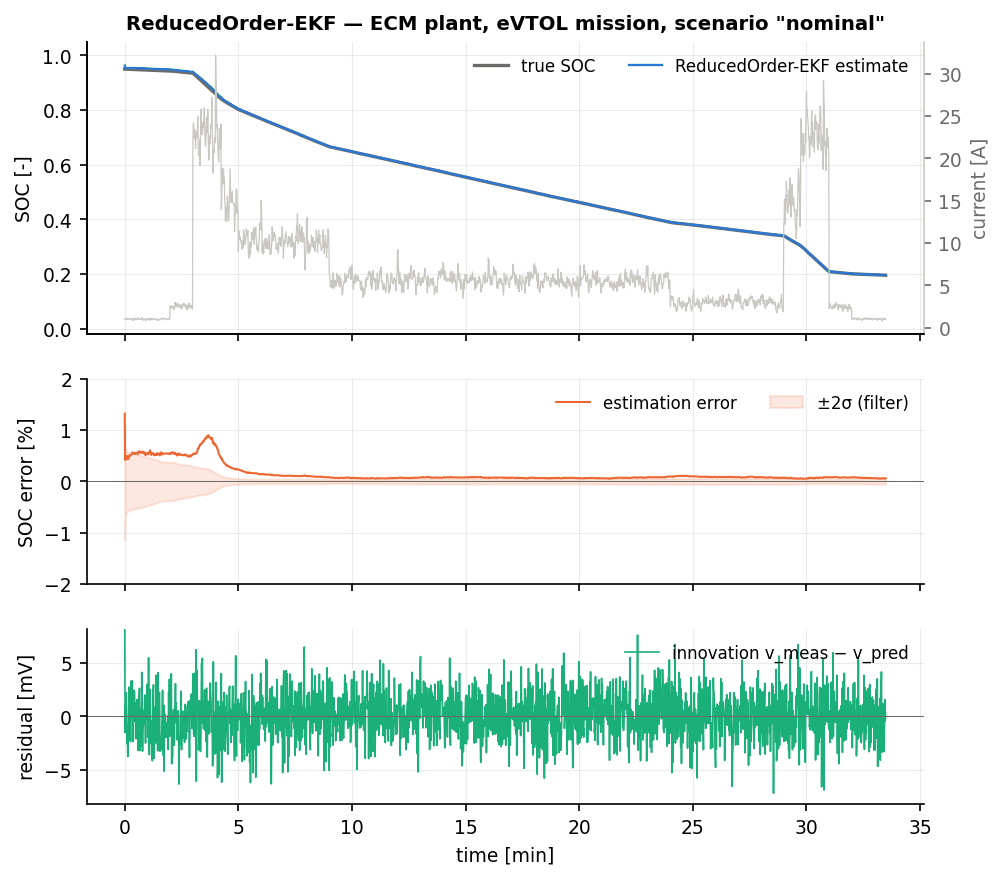
\includegraphics[width=\textwidth]{figures/cell_ReducedOrderEKF_nominal.png}
\caption{ReducedOrder-EKF on the nominal eVTOL mission: true and estimated SOC (top), estimation
error with the $\pm2\sigma$ band (middle), voltage residual (bottom).}
\end{figure}
\begin{figure}[H]\centering
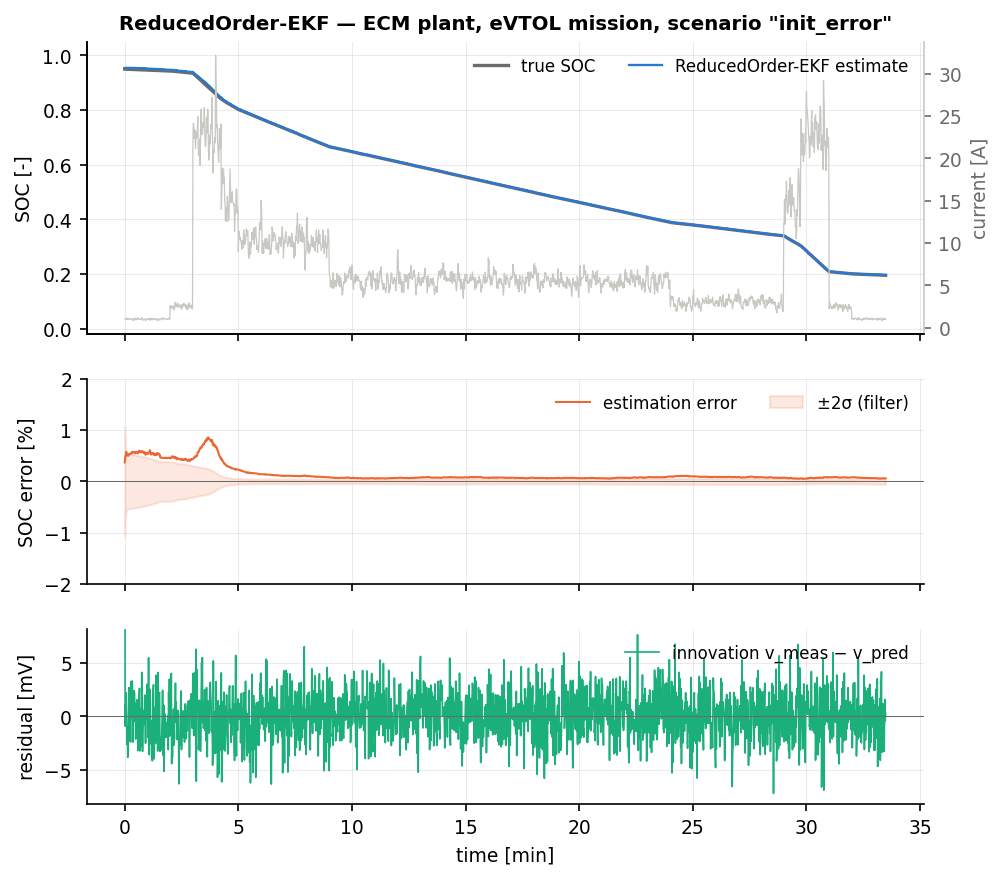
\includegraphics[width=\textwidth]{figures/cell_ReducedOrderEKF_init_error.png}
\caption{ReducedOrder-EKF with a 35\,\% initial SOC error.}
\end{figure}
\begin{figure}[H]\centering
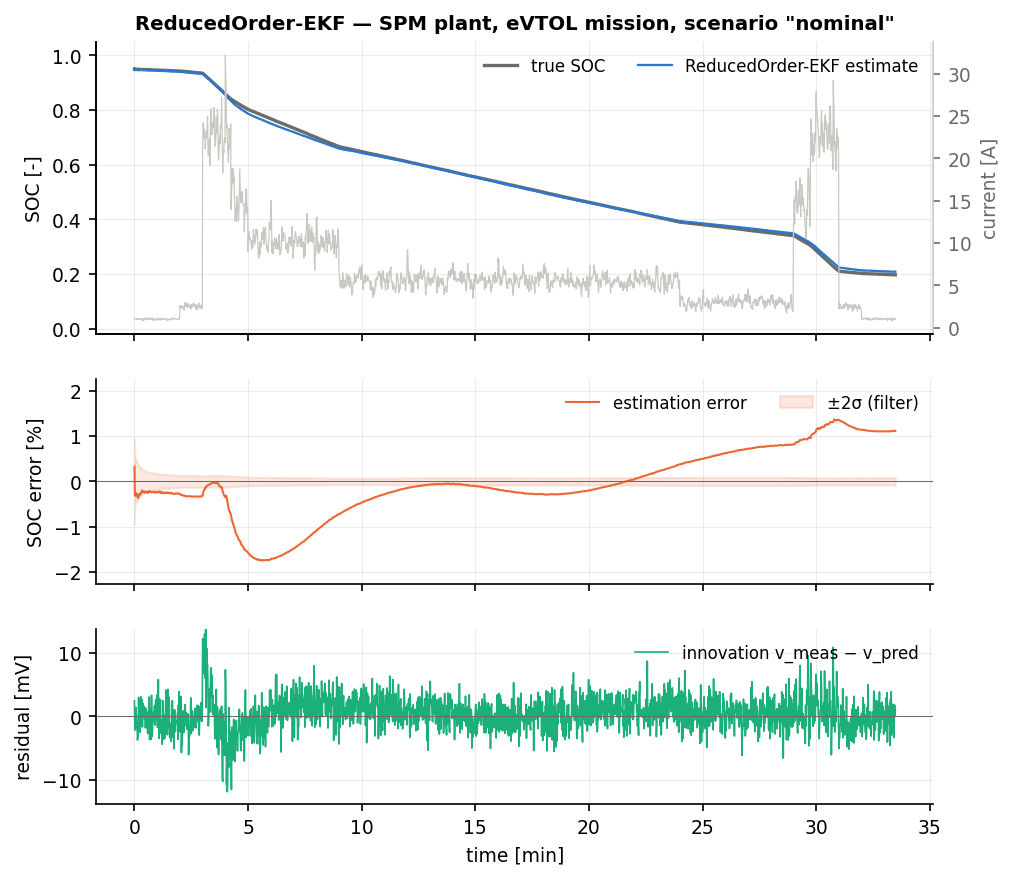
\includegraphics[width=\textwidth]{figures/cellspm_ReducedOrderEKF_nominal.png}
\caption{ReducedOrderEKF on the SPM (electrochemical) plant, nominal eVTOL mission.  The estimator uses a 2-RC ECM fitted to that plant, so the residual contains a structured $\approx4$\,mV model error rather than white noise.}
\end{figure}

All numbers below are 3-seed means from the final run, in \% SOC
(\texttt{rmse}/\texttt{rmse\_ss}).

\paragraph{ECM plant, eVTOL mission.}
\begin{center}\small
\begin{tabular}{@{}lccl@{}}
\toprule
Scenario & ReducedOrder-EKF & EKF ($n_x=4$) & Comment\\
\midrule
\texttt{nominal}        & $0.23/0.07$ & $0.15/0.05$ & $1.4\times$ worse --- the reduction cost\\
\texttt{init\_error}    & $0.22/0.07$ & $0.14/0.05$ & $t_\mathrm{conv}=0$\,s\\
\texttt{current\_bias}  & $1.08/0.85$ & $0.54/0.61$ & $1.4\times$ worse\\
\texttt{noise\_step}    & $0.23/0.10$ & $0.18/0.12$ & steady state slightly better\\
\texttt{outliers}       & $0.89/\mathbf{0.08}$ & $0.52/0.21$ & ss $2.6\times$ better, max $4.8\,\%$\\
\texttt{cold}           & $0.41/0.33$ & $0.20/0.16$ & $2\times$ worse\\
\texttt{hot}            & $0.17/\mathbf{0.02}$ & $0.20/0.03$ & ---\\
\texttt{aged\_cell}     & $3.22/2.12$ & $1.18/1.52$ & $1.4\times$ worse\\
\texttt{param\_mismatch}& $2.24/1.53$ & $1.28/1.36$ & $1.1\times$ worse\\
\texttt{sensor\_dropout}& $\mathbf{0.53/0.07}$ & $0.72/0.46$ & $\mathbf{6.6\times}$ better (ss)\\
\texttt{preisach}       & $1.04/0.99$ & $0.58/0.20$ & $5\times$ worse --- see below\\
\texttt{combined}       & $\mathbf{4.03/1.69}$ & $16.02/12.44$ & $\mathbf{7.4\times}$ better (ss); converges at 576\,s\\
\midrule
\multicolumn{2}{@{}l}{\textbf{ns/step}} & & $\mathbf{331}$ vs.\ $478$ ($-31\,\%$)\\
\multicolumn{2}{@{}l}{\textbf{$n_x$-dependent RAM}} & & $\mathbf{136}$\,B vs.\ $208$\,B ($-35\,\%$)\\
\bottomrule
\end{tabular}
\end{center}
Acceptance is met: \texttt{nominal} $\texttt{rmse\_ss}=0.07\,\%<2\,\%$, \texttt{init\_error}
$t_\mathrm{conv}=0$\,s, no divergence anywhere, worst ECM steady-state error $2.12\,\%$
(\texttt{aged\_cell}).

\paragraph{The accuracy cost.}  On clean data the reduced filter is $1.4\times$ less accurate in
steady state ($0.07\,\%$ vs.\ $0.05\,\%$).  Two mechanisms contribute and they can be separated:
with $\sigma_{v2}=0$ the single-seed nominal steady-state error is the same $0.08\,\%$, so the
inflated $\mR$ of \eqref{eq:ro-R} is \emph{not} the dominant term.  The rest comes from the loss of
the $v_2$ correction: the full EKF does use the measurement to adjust $v_2$ and, although that
adjustment is mostly noise, part of it correctly absorbs process-noise energy that the reduced
filter must now absorb through $\soc$.  The cost is largest where the slow branch matters most ---
\texttt{cold} ($2\times$: at $-10$\,\ensuremath{{}^\circ}C the Arrhenius factors make $R_2$ five
times and $\tau_2$ nearly four times their $25$\,\ensuremath{{}^\circ}C values, so the slow branch
reaches $\approx0.14$\,V during the take-off hover and its reconstruction error is the largest term
in the residual), \texttt{aged\_cell} ($1.4\times$) and \texttt{current\_bias} ($1.4\times$, where
a steady current offset produces a steady $v_2$ offset that the full filter can partly absorb).

\paragraph{Preisach.}  With the corrected plant sign convention \texttt{preisach} has become the
reduced model's worst relative result: $0.99\,\%$ against the EKF's $0.20\,\%$, and 77\,s to
converge against 16\,s.  The Preisach residual is a slowly varying voltage offset with no
current-proportional signature, i.e.\ exactly the shape that the full model's $v_2$ state can
absorb and the reduced model's fixed low-pass cannot.  This is the clearest single demonstration in
the chapter of what the dropped degree of freedom was actually doing: it was a low-frequency
residual sink, useful when the residual really is low-frequency and harmless noise otherwise.

\paragraph{The unexpected benefit.}  On \texttt{combined} the reduced filter is $7.4\times$ better
in steady state than the full EKF, on \texttt{sensor\_dropout} $6.6\times$ and on the steady-state
part of \texttt{outliers} $2.6\times$.  This is not the reduction being ``more accurate''; it is a
robustness effect and it is the same mechanism as the preceding paragraph read with the opposite
sign.  The full EKF's $v_2$ state is a free parameter with a very long time constant and almost no
observability, so when a large voltage residual appears --- the 200\,mV resistance error of the
aged cold cell, a 15\,s frozen sensor, a $\pm50$\,mV spike --- the filter has two ways to explain it
and the linearised update distributes the correction between $\soc$ and $v_2$ according to $\mP$,
not to physics.  Removing $v_2$ from the state removes that degree of freedom: the reduced filter
\emph{cannot} misattribute, so it degrades more gracefully.  Its \texttt{outliers} whole-run RMSE
($0.89\,\%$) and peak ($4.8\,\%$) are nevertheless worse than the EKF's, because a spike now has
nowhere to go but into $\soc$; the damage is transient, which is why the steady-state figure is the
better one.

\paragraph{SPM (electrochemical) plant.}  This is where the reduced model earns its place.  On the
SPM rows it gives $0.74/0.70\,\%$ on \texttt{nominal} against the EKF's $3.65/3.73\,\%$ --- a factor
of $5.3$ --- and it is essentially insensitive to the scenario: $0.70\,\%$ on \texttt{init\_error},
$0.71\,\%$ on \texttt{noise\_step}, $0.70\,\%$ on \texttt{outliers}, $0.70\,\%$ on
\texttt{sensor\_dropout} (against the EKF's $5.31\,\%$, $7.6\times$), $0.85\,\%$ on
\texttt{current\_bias} (against $5.69\,\%$, $6.7\times$), $0.64\,\%$ on \texttt{hot}.  Only
\texttt{cold} ($3.71\,\%$ vs.\ $7.35\,\%$) and \texttt{param\_mismatch} ($1.31\,\%$ vs.\
$3.13\,\%$) are above $1\,\%$.  Together with the Schmidt-KF ($0.51\,\%$) it is one of only two
filters in the family that break the $\approx3.7\,\%$ barrier at which every other estimator sits.

The mechanism is precisely the one identified above, now acting on a real model error rather than a
fault.  The SPM plant's $\approx4$\,mV structured residual is dominated by the concentration
overpotential, a slow, current-driven signal with a $\tau\approx556$\,s time constant --- which is
to say, it looks exactly like a slow RC branch that the fitted ECM does not get right.  A full 2-RC
EKF has a state, $v_2$, whose signature is indistinguishable from that residual over any window in
which the measurement is informative, and also indistinguishable from a slow drift in $\ocv(\soc)$.
Given a persistent residual of that shape the filter must split it between $v_2$ and $\soc$, and
because $\mP_{\soc\soc}$ is the larger of the two most of it lands on the SOC: hence the uniform
$3.1$--$4.1\,\%$ bias of the EKF and of every filter that keeps the fourth state.  The reduced model
has no $v_2$ to confuse with $\soc$; the slow branch is pinned to its open-loop value, the ambiguity
is structurally absent, and the residual is simply absorbed by the (deliberately inflated) $\mR$
instead of by the state.  The Schmidt-KF reaches the same place by a different route --- it inflates
$\mS$ so the ambiguous direction is never excited --- which is why those two, and only those two,
are immune.

The general lesson for model-order reduction is therefore stronger than the usual
flops-versus-accuracy trade: on a plant whose unmodelled physics resembles the state you removed,
removing it is not merely cheap but \emph{more accurate}, because a weakly observable state is a
liability in exactly the situation where the model is wrong.


\section{Summary}
Removing the slow RC branch from the estimator state and reconstructing it open loop costs
$1.4\times$ in steady-state SOC accuracy on clean ECM data and buys a $31\,\%$ reduction in CPU
time and a $35\,\%$ reduction in per-cell RAM --- the single cheapest way in this library to fit an
EKF-class estimator into a small MCU budget for a large pack, and the only estimator here that is
faster than the plain EKF.  It also, far from unexpectedly once the mechanism is understood, makes
the filter dramatically more robust wherever the residual is a slow, current-driven signal that the
missing state could have absorbed: $7.4\times$ better than the EKF on \texttt{combined} and
$5.3\times$ better on the electrochemical plant, where it and the consider filter are the only two
methods in this family that escape the $\approx3.7\,\%$ model-error floor.  Use it when the number
of cells, not the accuracy per cell, is the binding constraint; when the plant is richer than the
2-RC model used to estimate it; and when the mission has no long rests.  Do not use it when the
slow branch is genuinely observable (a chemistry with $\tau_2\approx20$\,s, a mission with
20-minute rests), where the \texttt{preisach} result --- $5\times$ worse than the full model --- is
the warning, and never with sigma-point or particle filters: the quasi-static branch is advanced
inside $\vf$ and assumes exactly one evaluation per sampling period.
